% This is samplepaper.tex, a sample chapter demonstrating the
% LLNCS macro package for Springer Computer Science proceedings;
% Version 2.21 of 2022/01/12
%
\documentclass[runningheads]{llncs}

\usepackage{float}
%
\usepackage[T1]{fontenc}
% T1 fonts will be used to generate the final print and online PDFs,
% so please use T1 fonts in your manuscript whenever possible.
% Other font encondings may result in incorrect characters.
%
\usepackage[super, square]{natbib}

\usepackage[dvipsnames]{xcolor}
\usepackage{hyperref}
\hypersetup{
    colorlinks=true,
    linkcolor=black,
    citecolor=CadetBlue,
    filecolor=CadetBlue,      
    urlcolor=CadetBlue,
}
\usepackage{graphicx}
% Used for displaying a sample figure. If possible, figure files should
% be included in EPS format.
%
% If you use the hyperref package, please uncomment the following two lines
% to display URLs in blue roman font according to Springer's eBook style:
\usepackage{color}
%\renewcommand\UrlFont{\color{blue}\rmfamily}
%\urlstyle{rm}
%

\usepackage{longtable}


\begin{document}

\title{Survey on Energy Consumption Optimization Approach in Container-Based Cloud Environments}
\titlerunning{Energy Optimization in Container-Based Cloud Environments}


\author{Francesco Pace Napoleone\inst{1} \and
Marian-Catalin Mutu-Costan\inst{1} \and
Ihor Ryzhuk\inst{1} \and
Ewan Soueidan\inst{1}}

\authorrunning{F. Pace Napoleone et al.}

\institute{Université de Toulouse, France \\
\email{\{francesco.pace-napoleone, marian.mutu-costan, ihor.ryzhuk, ewan.soueidan\}@univ-tlse3.fr}}

\maketitle
%
\begin{abstract}

Growing demand for cloud services has shifted data center design from performance-centric to energy-efficient architectures. Containerization, a lightweight alternative to virtual machine, enables flexible resource allocation and reduced overhead. This survey reviews energy optimization techniques in container-based cloud environments by systematically selecting studies from 2010-2020 and categorizing them by scheduling scope, optimization method, energy-saving strategy, and Docker maturity. Our analysis covers early VM consolidation methods that achieved up to 83\% energy savings, predictive scheduling, and advanced container orchestration. Overall, container-based optimizations, particularly those leveraging AI and hybrid heuristics, significantly reduce energy consumption while maintaining Quality of Service (QoS), pointing to promising future research directions.

\keywords{Cloud Computing \and Containerization \and Energy Optimization \and Microservices \and Resource Allocation
}
\end{abstract}

\section{Introduction}

\subsection{Background and Motivation}
Cloud computing evolved to support scalable platform usage, moving from single-file applications to client/server 
architectures with monolithic backends, then to microservices with containers, and now transitioning to micro-frontends. 
Containers run directly on the host using Linux CGroups, bypassing the hypervisor overhead inherent in VMs (e.g., 
Proxmox, VMWare), which allows for full utilization of host CPU resources and simplifies telemetry monitoring. 
This lightweight nature is evident in Docker files that simply copy files and run builds, making containers easier to integrate 
into CI/CD pipelines.

However, this increased reliance on cloud-based infrastructures has led to a significant rise in energy 
consumption. In 2006, the electricity costs for IT infrastructures in the United States alone were 
estimated at \$4.5 billion\cite{beloglazov_energy_2010}. Energy consumption optimization has since become a 
critical concern, especially as cloud data centers now account for approximately 1-1.5\% of global 
electricity use\cite{IEADataCentres}. Despite efficiency improvements, the demand for digital 
services continues to grow, pushing the need for more sustainable solutions.

\subsection{Research Trends and Contributions}
Early research focused on heuristic-based approaches to optimize virtual machine (VM) placement, achieving 
energy savings of up to 83\% while maintaining only a 1.1\% service level agreement (SLA) violation 
rate\cite{beloglazov_energy_2010}. More recently, research has shifted from VM-based allocation towards 
containerized environments, where energy efficiency is influenced by scheduling strategies, workload 
distribution, and infrastructure optimizations. 

The paper ``Survey on Energy Consumption Optimization Approach in Container Based Cloud Environments'' 
further highlights that containerization not only drives scalability and 
reproducibility but also plays a crucial role in optimizing energy consumption. It 
explores strategies for efficient resource allocation, reducing power overhead, and 
ensuring that the benefits of container-based deployments extend beyond performance 
to sustainability in cloud infrastructures.
In this work, we present a state-of-the-art review on Energy Consumption Optimization Approaches in 
Container-Based Cloud Environments. Our survey of the available literature—predominantly spanning 
from 2010 to 2020—reveals that foundational research primarily focused on energy measurement, 
basic optimization strategies, and energy visualization techniques\cite{beloglazov_energy_2010}.

Early contributions, such as those by Beloglazov and Buyya\cite{beloglazov_energy_2010}, as well as 
Piraghaj et al.\cite{piraghaj_framework_2015}, laid the groundwork for dynamic resource allocation and 
energy-efficient container consolidation. Later advancements introduced more sophisticated container 
scheduling mechanisms, including availability-aware scheduling\cite{alahmad_availability-aware_2018}, 
concurrent scheduling in heterogeneous clusters\cite{hu_concurrent_2020}, and hybrid AI-driven resource 
allocation\cite{tan_hybrid_2019}.
In parallel, energy-efficient resource management techniques gained prominence, incorporating renewable 
energy-aware scheduling\cite{kumar_renewable_2019}, optimization-based consolidation methods\cite{shi_energy-aware_2018, piraghaj_framework_2015}, 
and brownout-based scheduling strategies\cite{xu_energy_2016}. Several studies further explored 
predictive optimization and SLA-aware provisioning frameworks to enhance energy 
efficiency\cite{dabbagh_energy-efficient_2015, hameed_survey_2016, li_sla-aware_2018, bui_energy_2017, 
carrega_energy-aware_2017}.

Beyond optimization techniques, researchers have also examined broader energy consumption trends and policy implications\cite{avgerinou_trends_2017}, 
reflecting the increasing emphasis on sustainability in cloud computing. Additionally, efforts in DevOps-driven elastic container management have contributed 
to improving the adaptability and efficiency of containerized cloud applications\cite{barna_delivering_2017}.
Although these prior works have significantly advanced the field, our review highlights an evolving trend toward more integrated and user-centric energy 
management strategies, as reflected in recent data on energy consumption in cloud environments\cite{masanet_2020, hintemann_2022, IEADataCentres}.

\section{Methodology}
The research process began by defining our scope together with our supervisor, Professor Jean-Marc Pierson. We focused on creating a state-of-the-art review 
addressing energy consumption optimization within Container and Cloud Computing.

Initially, we defined a structured ``Search Pipeline'' illustrated in Figure~\ref{fig:search_pipeline}, ensuring systematic identification and evaluation of relevant papers.

\begin{figure}[H]
    \centering
    \includegraphics[width=0.8\columnwidth]{flowchartTIR.png}
    \caption{Search Pipeline Flowchart}\label{fig:search_pipeline}
\end{figure}

We developed an initial search query: \textit{((energy OR resource) AND container)}, including ``resource'' to account for better resource utilization directly influencing energy efficiency.

Clear exclusion criteria were established beforehand (Table~\ref{tab:Exclusion Rules}), filtering out irrelevant work and focusing exclusively on impactful research.
\begin{table}[H]
\centering
\begin{tabular}{c}
\hline
Direct Exclusion of Paper If \\ \hline
Work is not in English \\ 
Work is not a scientific paper \\ 
Work has fewer than 10 citations \\ 
Work is not related to containers/cloud \\ \hline
\end{tabular}
    \caption{Exclusion Criteria}
    \label{tab:Exclusion Rules}
\end{table}

This approach yielded 34 relevant papers, sourced across various publishers, as depicted in Figure~\ref{fig:exported_papers}.

\begin{figure}[H]
    \centering
    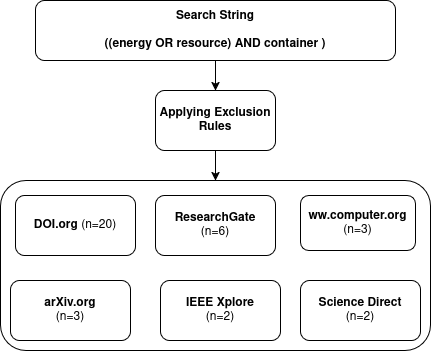
\includegraphics[width=0.7\columnwidth]{exportedPapers.png}
    \caption{Distribution of Exported Papers by Publisher}\label{fig:exported_papers}
\end{figure}

The majority of selected studies were published between 2017 and 2019 (Figure~\ref{fig:papers_per_year}), reflecting a peak period of research interest.

\begin{figure}[H]
    \centering
    \includegraphics[width=0.7\columnwidth]{papers_per_year.png}
    \caption{Papers per Year}\label{fig:papers_per_year}
\end{figure}

After paper selection, we defined specific classification metrics (Table~\ref{tab:Paper Classification}) to analyze the technical dimensions of energy-aware scheduling approaches.

\begin{table}[H]
\centering
\begin{tabular}{c}
\hline
Classification Categories\\ \hline
Optimization Technique \\ 
Target Level  \\ 
Scheduling Scope \\ 
Energy Strategy \\
Docker Awareness \\
\hline
\end{tabular}
    \caption{Paper Classification Metrics}
    \label{tab:Paper Classification}
\end{table}

The classification categories are defined as follows:
\begin{itemize}
  \small
  \item \textbf{Scheduling Scope}
    \begin{itemize}
      \item \textbf{Online}: Decisions at runtime.
      \item \textbf{Offline}: Known workload beforehand.
      \item \textbf{Predictive}: Forecast-based decisions.
      \item \textbf{Reactive}: Triggered by SLA violations or thresholds.
      \item \textbf{Concurrent}: Simultaneous multiple-task scheduling.
    \end{itemize}

  \item \textbf{Optimization Technique}
    \begin{itemize}
      \item \textbf{Greedy}: Stepwise local decisions.
      \item \textbf{Model-Based}: Predictive analytical models.
      \item \textbf{PSO}: Bio-inspired global optimization.
      \item \textbf{Evolutionary}: Genetic/evolution-based methods.
      \item \textbf{Meta-Heuristic}: High-level heuristic strategies.
      \item \textbf{MCMF}: Flow-network optimization.
    \end{itemize}

  \item \textbf{Energy Strategy}
    \begin{itemize}
      \item \textbf{Consolidation}: Migrate to reduce active hosts.
      \item \textbf{Brownout}: Temporarily disable app components.
      \item \textbf{QoS Maintenance}: Energy-saving without SLA violations.
      \item \textbf{Renewable-aware}: Optimize for renewable energy availability.
    \end{itemize}

  \item \textbf{Docker Awareness}
    \begin{itemize}
      \item \textbf{Pre-Docker}: Pre-containerization (VM-only).
      \item \textbf{Early Docker}: Containers used like VMs.
      \item \textbf{Mature Docker}: Container-specific optimizations.
    \end{itemize}
\end{itemize}

We incorporated \textbf{Docker Awareness} to highlight the technological transition from virtual machines to containers, essential for understanding changes in scheduling complexity. \textbf{Energy Awareness} is included to represent approaches' capability to balance energy efficiency with QoS constraints, recognizing the different trade-offs between performance and sustainability.

Finally, Tables~\ref{tab:technical_papers} and \ref{tab:surveys} summarize our classified selection, and Figure~\ref{fig:trend_analysis} visually correlates scheduling approaches with their publication years.

\begin{figure}[H]
    \centering
    \includegraphics[width=1\linewidth]{Trend_Analysis.jpeg}
    \caption{Trend Analysis}
    \label{fig:trend_analysis}
\end{figure}

\begin{footnotesize}
\begin{longtable}{|p{3.8cm}|p{2.3cm}|p{1.6cm}|p{2.3cm}|p{2.2cm}|p{2cm}|}
\hline
\textbf{Paper Ref.} & \textbf{Optimization Technique} & \textbf{Target Level} & \textbf{Scheduling Scope} & \textbf{Energy Strategy} & \textbf{Docker Awareness} \\
\hline
\endfirsthead

\hline
\textbf{Paper Ref.} & \textbf{Optimization Technique} & \textbf{Target Level} & \textbf{Scheduling Scope} & \textbf{Energy Strategy} & \textbf{Docker Awareness} \\
\hline
\endhead
Availability-Aware Scheduler\cite{alahmad_availability-aware_2018} (2018) & Greedy & Container, VM & Offline & Availability & Mature Docker\\
\hline
Renewable-Aware Scheduling\cite{kumar_renewable_2019} (2019)& Greedy & Container, VM & Reactive & Consolidation & Mature Docker \\
\hline
Concurrent Container Scheduling\cite{hu_concurrent_2020} (2020)& MCMF & Container & Concurrent & Consolidation & Mature Docker \\
\hline
GP Hyper-Heuristic for Containers\cite{tan_hybrid_2019} (2019)& Evolutionary & Container, VM & Online & Consolidation & Mature Docker \\
\hline
PSO-Based Container Consolidation\cite{shi_energy-aware_2018} (2018)& PSO & Container & Offline & Consolidation & Mature Docker \\
\hline
Energy-Efficient Container Framework\cite{piraghaj_framework_2015} (2015)& Greedy & Container, VM & Reactive & Consolidation & Early Docker \\
\hline
VM Consolidation Strategy\cite{carrega_energy-aware_2017} (2017)& Meta-Heuristic & VM & Online & Consolidation & Mature Docker \\
\hline
Predictive Resource Provisioning\cite{dabbagh_energy-efficient_2015} (2015)& Model-based  & VM & Predictive & Consolidation & Early-Docker \\
\hline
Dynamic VM Reallocation\cite{beloglazov_energy_2010} (2010) & Greedy & VM & Online & Consolidation & Pre-Docker \\
\hline
Autonomic Container Management\cite{barna_delivering_2017} (2017) & Model-based & Container, VM & Predictive & QoS & Mature Docker \\
\hline
Brownout-Based Scheduling\cite{xu_energy_2016} (2016)& Greedy & Application Layer & Reactive & Brownout & Mature Docker \\
\hline
GPR + Convex VM Planning\cite{bui_energy_2017} (2017) & Model-Based & VM, PM & Predictive & Consolidation & Mature Docker \\
\hline
SLA-Aware Consolidation\cite{li_sla-aware_2018} (2018) & Model-Based & VM, PM & Predictive & Consolidation & Mature Docker \\
\hline
\caption{Classification of Technical Papers on Energy-Aware Scheduling}
\label{tab:technical_papers}
\end{longtable}
\end{footnotesize}

\begin{table}[H]
\centering
\footnotesize
\begin{tabular}{|p{5.5cm}|p{3.5cm}|p{4cm}|}
\hline
\textbf{Paper Ref.} & \textbf{Type} & \textbf{Scope / Focus} \\
\hline
Survey on Energy-Aware Scheduling\cite{hameed_survey_2016}  & Survey & Overview of VM and container-level techniques \\
\hline
Global Energy Estimates\cite{masanet_2020} & Analysis & Environmental impact of data centers \\
\hline
Cloud Impact on Energy\cite{hintemann_2022} & Report & Energy use in European data centers \\
\hline
IEA Report on Data Centers\cite{IEADataCentres} & Report & Global energy trends in ICT and data centers \\
\hline
EU Data Center Energy Trends\cite{avgerinou_trends_2017} & Analysis & EU-level trends in ICT energy consumption \\
\hline
\end{tabular}
\caption{Survey and Analysis Papers}
\label{tab:surveys}
\end{table}

\section{Trend reconstruction}

\subsection{Early approaches}
Early approaches date back to 2010, with Docker being released in 2013. In 2006, the cost of electricity consumed by IT infrastructures in the US was estimated at 4.5 billion dollars and was projected to double by 2011 \cite{beloglazov_energy_2010}.

In the initial attempts described in\cite{beloglazov_energy_2010}, a simple Bin Packing variation with dynamic voltage and frequency scaling (DVFS) enabled was used to address this problem. The results, obtained using the CloudSim environment, showed an energy savings gain of 83\% compared to no policy, with an SLA violation of 1.1\%. This marked the beginning of research in this area.

By 2015, researchers shifted toward predictive modeling to overcome the limitations of static thresholds. In \cite{dabbagh_energy-efficient_2015},
a Wiener filter-based predictor was introduced to estimate cluster workloads, 
combined with Best Fit Decreasing for physical machine allocation.
This approach improved energy efficiency by up to 33\% compared to heuristic methods.
Shortly after, in 2017, further improvements were made to predictive models \cite{bui_energy_2017}.
This work extended previous research by incorporating Gaussian Process Regression (GPR) for non-stationary workload prediction,
accelerated using the Fast Fourier Transform to mitigate GPR's computational complexity.
Additionally, a convex optimization-based migration strategy was employed.
These enhancements resulted in a 35\% energy efficiency improvement over heuristic methods, with only a 15\% latency tradeoff.

\subsection{From Virtual Machines to Containers}

As cloud infrastructures evolve, the shift from VM-based to container-based deployments has become central to achieving energy efficiency and maintaining SLA compliance. Containers offer a lightweight alternative to VMs, reducing overhead and enabling more flexible resource allocation\cite{alahmad_availability-aware_2018}. Early container-based systems focused on reducing active VM counts through migration techniques—employing modular watchdogs and Pearson correlation checks to optimize resource usage\cite{alahmad_availability-aware_2018}.

Subsequent research advanced container scheduling by using flow network models to frame the allocation problem as a minimum cost flow problem. This approach effectively balances multi-resource constraints (e.g., CPU and memory) and has proven scalable in simulations involving up to 5000 machines\cite{hu_concurrent_2020}. 

More recent hybrid methods, which combine evolved rules from genetic programming with human-designed heuristics, address the two-level allocation challenge (assigning containers to VMs and VMs to physical machines). These techniques not only enhance energy efficiency but also improve fault tolerance by incorporating reliability metrics such as Mean Time To Failure (MTTF) and Mean Time To Repair (MTTR)\cite{tan_hybrid_2019, alahmad_availability-aware_2018}. Complementary studies, such as those by Kumar et al.\cite{kumar_renewable_2019} and Shi et al.\cite{shi_energy-aware_2018}, further demonstrate that container-based approaches can significantly reduce energy consumption and improve overall system performance.

This evolution—from basic migration techniques to advanced, hybrid scheduling—forms a critical foundation for the energy optimization and resilience strategies.

\section{Method Analysis}

\subsection{Methodology}

Over time, different researchers have utilized various testing environments and hardware configurations to evaluate their energy-aware scheduling algorithms. To examine the evolution of their experimental approaches, we have collected and structured data from the selected papers, focusing on the simulation environment, the number of CPU Cores, memory capacity, and power consumption of the experimentation hardware. Specifically, we define:

\begin{itemize}
    \footnotesize
    \item \textbf{P idle (W)} as the power consumption at low CPU utilization (generally below 50\% load).
    \item \textbf{P max (W)} as the power consumption at maximum CPU load.
\end{itemize}

In some studies, multiple hardware configurations were reported—either due to hardware availability or to assess performance on more powerful setups. In these cases, multiple entries are provided in the table. Note that when power consumption figures were not experimentally reported but instead obtained from hardware specification (by searching for the make and model), those values are marked with an asterisk (\textasteriskcentered). Whenever certain data fields were omitted by the authors, we use ``Nm'' (not mentioned).

\begin{footnotesize}
\begin{longtable}{|p{3.8cm}|p{2.2cm}|p{1.2cm}|p{1.5cm}|p{1.8cm}|p{1.8cm}|}
\hline
\textbf{Paper Ref.} & \textbf{Simulation Environment} & \textbf{CPU Cores} & \textbf{Memory (GB)} & \textbf{Power P idle (W)} & \textbf{Power P max (W)} \\
\hline
\endfirsthead

\hline
\textbf{Paper Ref.} & \textbf{Simulation Environment} & \textbf{CPU Cores} & \textbf{Memory (GB)} & \textbf{Power P idle (W)} & \textbf{Power P max (W)} \\
\hline
\endhead
Availability-Aware Scheduler \cite{alahmad_availability-aware_2018} (2018) & CloudSim & Nm & Nm & Nm & Nm \\
\hline
Renewable-Aware Scheduling \cite{kumar_renewable_2019} (2019) & Nm & 4 & 64 & 100 & 150 \\
\hline
Renewable-Aware Scheduling \cite{kumar_renewable_2019} (2019) & Nm & 8 & 128 & 120 & 200 \\
\hline
Renewable-Aware Scheduling \cite{kumar_renewable_2019} (2019) & Nm & 16 & 256 & 150 & 250 \\
\hline
Concurrent Container Scheduling \cite{hu_concurrent_2020} (2020) Homogeneous Cluster & ExoGENI & 2 & 6 & Nm & Nm \\
\hline
Concurrent Container Scheduling \cite{hu_concurrent_2020} (2020) & ExoGENI & 1 & 3 & Nm & Nm \\
\hline
Concurrent Container Scheduling \cite{hu_concurrent_2020} (2020) & ExoGENI & 2 & 6 & Nm & Nm \\
\hline
Concurrent Container Scheduling \cite{hu_concurrent_2020} (2020) & ExoGENI & 4 & 12 & Nm & Nm \\
\hline
GP Hyper-Heuristic for Containers \cite{tan_hybrid_2019} (2019) & Nm & Nm & 0.8 & Nm & Nm \\
\hline
PSO-Based Container Consolidation \cite{shi_energy-aware_2018} (2018) & Nm & 4 & 16 & Nm & Nm \\
\hline
Energy-Efficient Container Framework \cite{piraghaj_framework_2015} & CloudSim & 4 & 64 & 86 & 117 \\
\hline
Energy-Efficient Container Framework \cite{piraghaj_framework_2015} & CloudSim & 8 & 128 & 93 & 135 \\
\hline
Energy-Efficient Container Framework \cite{piraghaj_framework_2015} & CloudSim & 16 & 256 & 66 & 247 \\
\hline
VM Consolidation Strategy \cite{carrega_energy-aware_2017} (2017) & Nm & 2 & Nm & 170 & 220 \\
\hline
Predictive Resource Provisioning \cite{dabbagh_energy-efficient_2015} (2015) & Nm & Nm & Nm & 107 & 300.81 \\
\hline
Dynamic VM Reallocation \cite{beloglazov_energy_2010} (2010) & Nm & 1 & 8 & Nm & Nm \\
\hline
Autonomic Container Management \cite{barna_delivering_2017} (2017) & LEGIS & Nm & 16 & Nm & Nm \\
\hline
Brownout-Based Scheduling \cite{xu_energy_2016} & CloudSim & 2 & 4 & 156\textasteriskcentered & 247\textasteriskcentered \\
\hline
GPR + Convex VM Planning \cite{bui_energy_2017} (2017) & Nm & 4 & 12 & 225\textasteriskcentered & 375\textasteriskcentered \\
\hline
SLA-Aware Consolidation \cite{li_sla-aware_2018} (2018) & CloudSim & 2 & 4 & 102 & 117 \\
\hline
SLA-Aware Consolidation \cite{li_sla-aware_2018} (2018) & CloudSim & 2 & 4 & 116 & 135 \\
\hline
\caption{Hardware and Power Specifications}
\label{tab:hardware_specs}
\end{longtable}
\end{footnotesize}

\subsection{Plots and Visualization}

We visualized the simulation environments used in each paper over time to observe how they have evolved (Figure~\ref{fig:timeline}). Each point corresponds to a paper, placed according to its publication year and the simulation platform it utilized (CloudSim, ExoGENI, LEGIS, or ``Nm'' if not mentioned) Each point denotes a paper, positioned by its publication year and the simulation platform it utilized.

\begin{figure}[H]
    \centering
    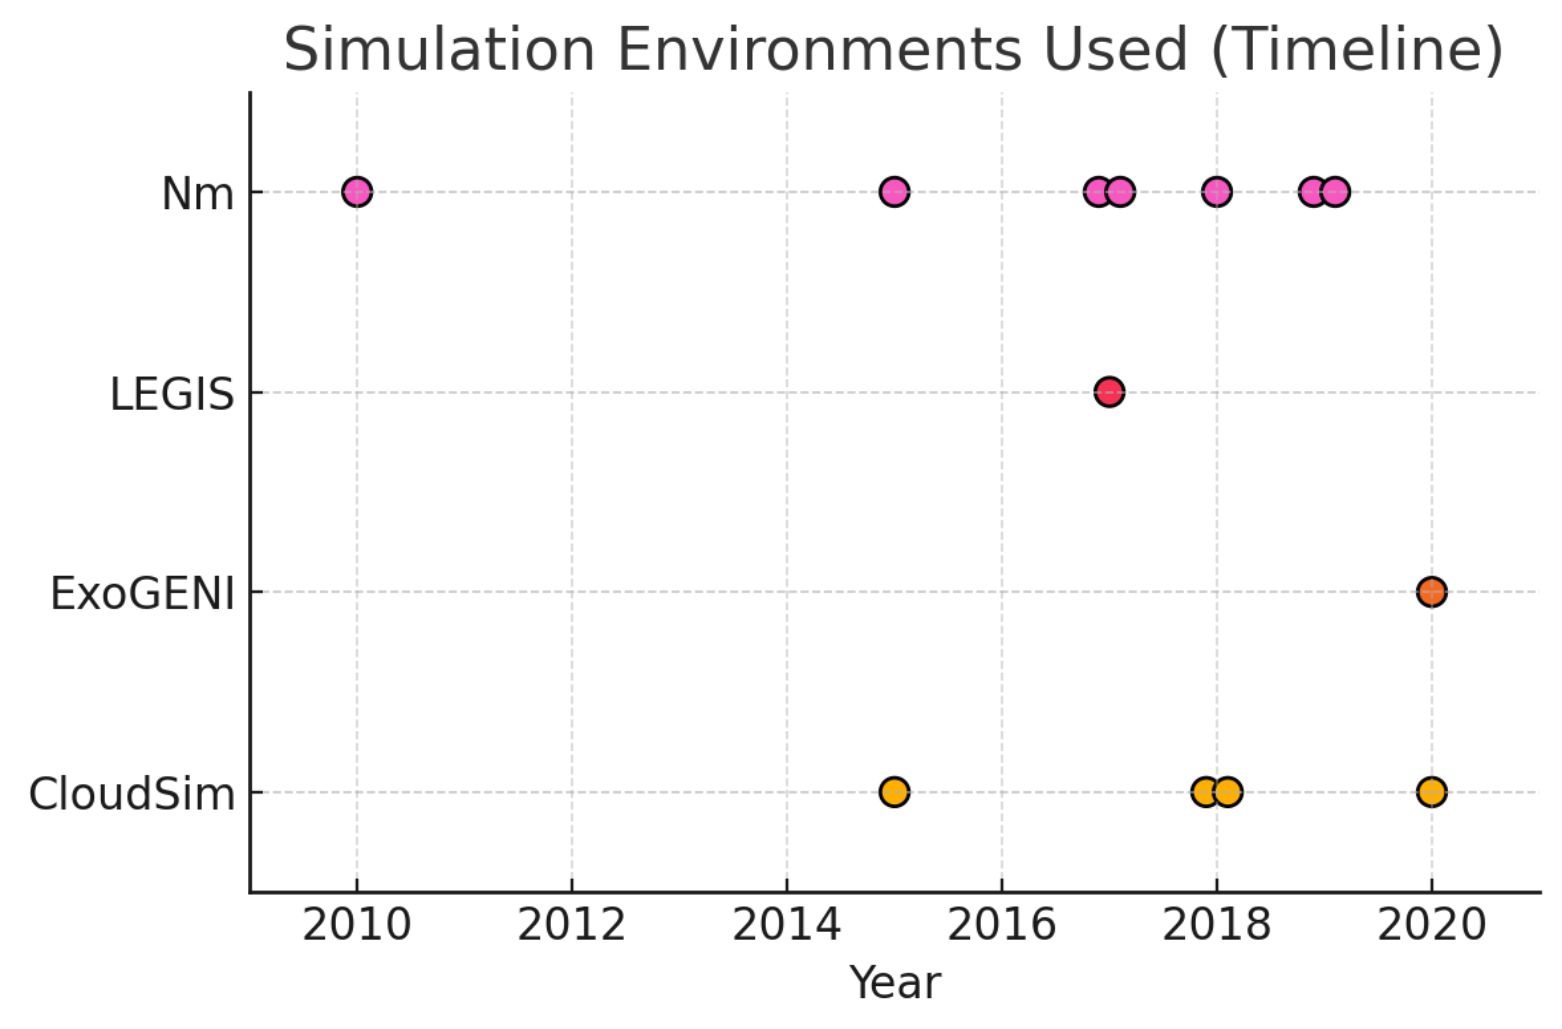
\includegraphics[width=0.7\columnwidth]{Timeline.png}
    \caption{Timeline of simulation environments used in each paper (2010--2020). }
    \label{fig:timeline}
\end{figure}

Additionally, we plotted the relationship between the number of CPU cores and the \textit{energy delta} (the difference $P_{\max} - P_{\begin{footnotesize}idle \end{footnotesize}}$), shown in Figure~\ref{fig:energy_delta}. This second figure highlights how dynamic power consumption scales with increased core counts and is further distinguished by algorithm type (color) and simulation environment (marker shape).

\begin{figure}[H]
    \centering
    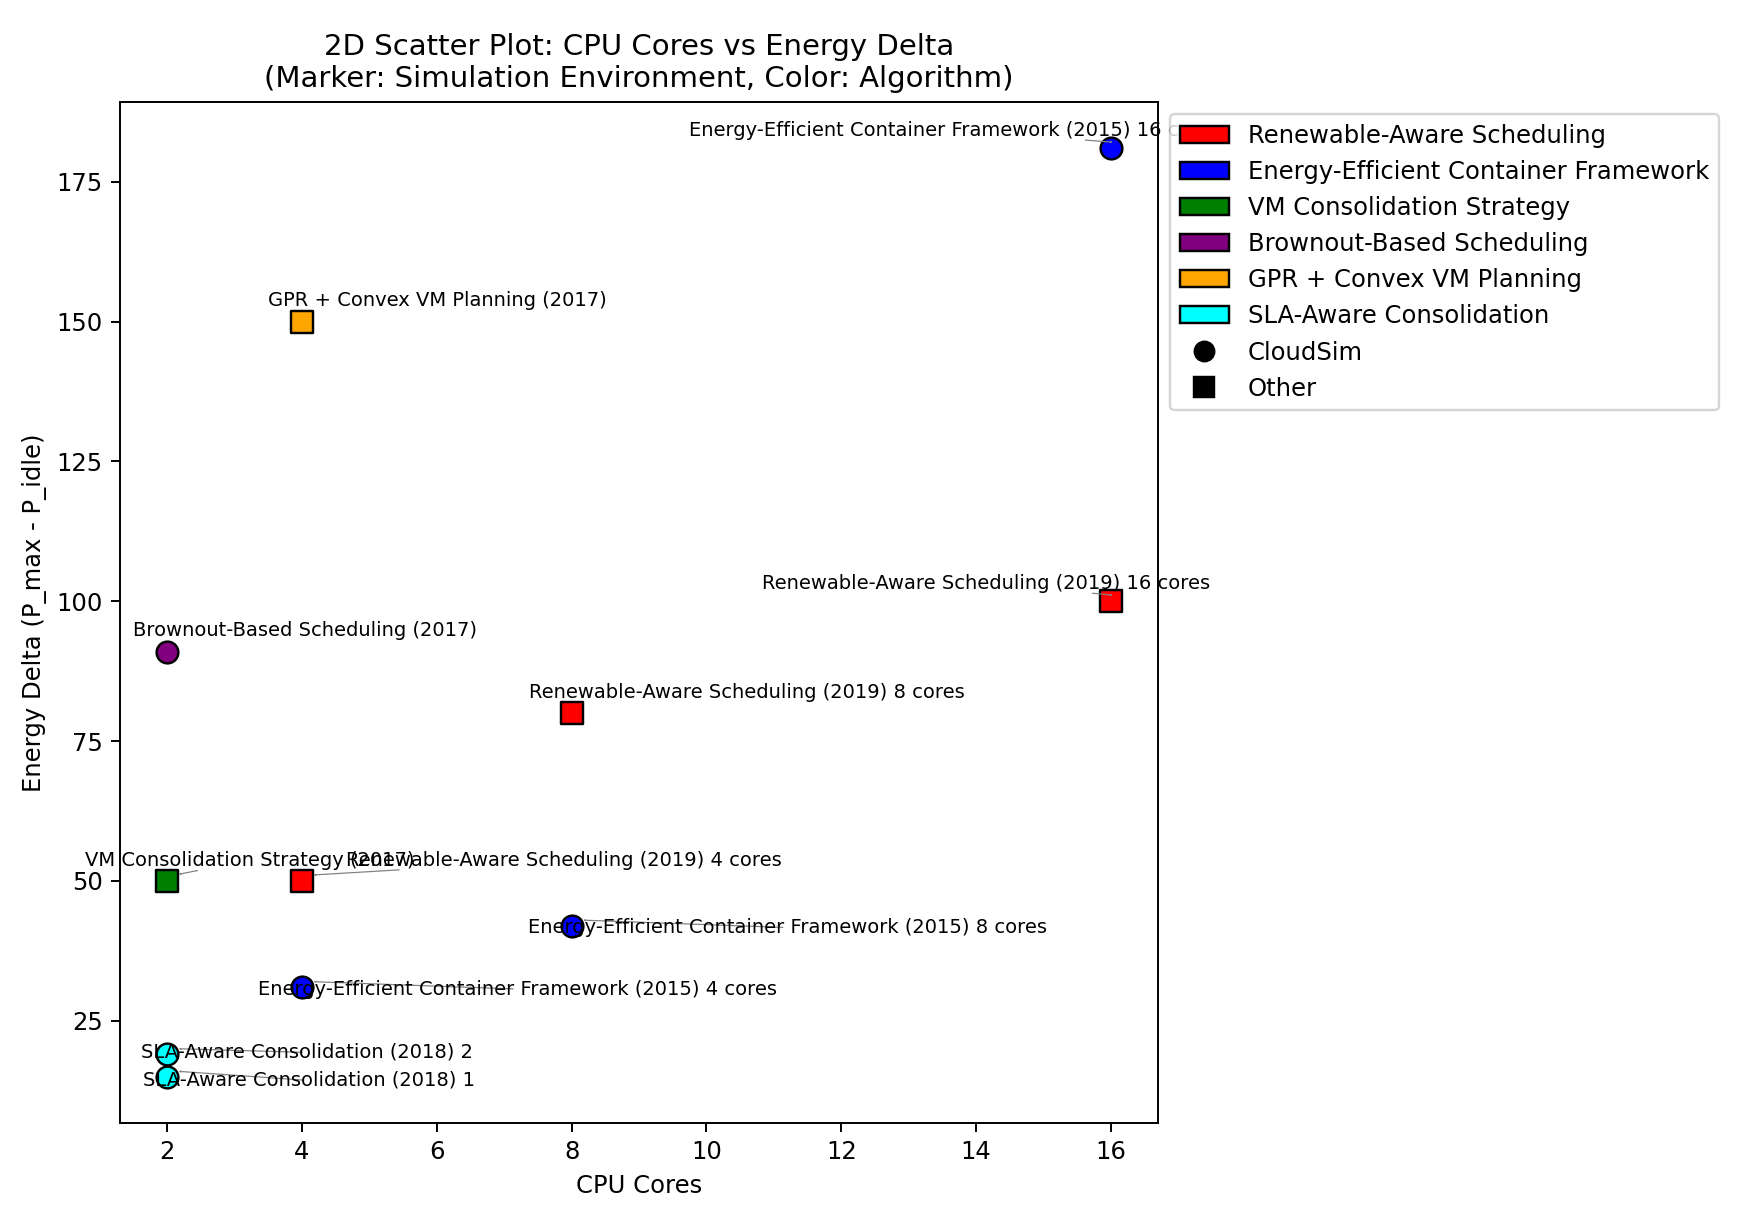
\includegraphics[width=0.75\columnwidth]{Energy.png}
    \caption{2D Scatter Plot: CPU cores vs. Energy Delta $(P_{\max} - P_{\begin{footnotesize}idle\end{footnotesize}})$.}
    \label{fig:energy_delta}
\end{figure}

\section{Conclusions}

Energy consumption optimization in container-based cloud environments has evolved from early heuristic methods to sophisticated, predictive, and container-aware scheduling approaches. Early consolidation techniques demonstrated significant energy savings through aggressive host shutdown and DVFS, but their reliance on static thresholds often limited adaptability under dynamic workloads\cite{carrega_energy-aware_2017}. In contrast, predictive algorithms that incorporate workload forecasting and dynamic resource allocation have achieved further energy reductions (typically 30--35\%) while balancing the trade-off between energy savings and service quality\cite{dabbagh_energy-efficient_2015,bui_energy_2017}.

The transition from VM-based to container-based solutions has enabled finer-grained resource management, with approaches such as flow-network optimization for container placement proving effective even in large-scale simulations\cite{hu_concurrent_2020}. Additionally, strategies like brownout scheduling\cite{xu_energy_2016} and meta-heuristic or AI-driven methods\cite{tan_hybrid_2019,shi_energy-aware_2018} have shown promise in achieving global optimization over complex infrastructures, albeit with increased computational overhead.

A key insight from the surveyed literature is that no single method outperforms all others under every scenario; instead, each approach excels in specific operational contexts. For instance, consolidation-focused strategies yield high energy savings but require careful management to avoid SLA violations, whereas QoS-aware methods maintain performance at the expense of some energy efficiency\cite{li_sla-aware_2018}. Moreover, the emerging integration of renewable energy awareness into scheduling algorithms\cite{kumar_renewable_2019} points toward a future where energy management is not only efficient but also environmentally sustainable.

Looking ahead, future research should aim to integrate these diverse techniques into hybrid frameworks that combine predictive scheduling, dynamic consolidation, and real-time QoS monitoring. This integration, alongside the continued evolution of container orchestration platforms, is essential for achieving the dual goals of operational efficiency and sustainable cloud computing.

\bibliographystyle{splncs04}
\bibliography{mybibliography}

\end{document}
